\documentclass[referee]{USG}
\usepackage{amsmath,amssymb,booktabs,array,url,xcolor,graphicx,microtype,tikz}
\usetikzlibrary{arrows.meta,positioning,fit,calc}
\newcommand{\dauc}{\ensuremath{\Delta\mathrm{AUC}}}
\newcommand{\optm}{\ensuremath{\mathrm{optimism}}}
\newcommand{\uinner}{\ensuremath{U_{\mathrm{in}}}}
\newcommand{\uouter}{\ensuremath{U_{\mathrm{out}}}}
\graphicspath{{images/}{figures/}}

\begin{document}
\title{Search Breadth and Deployment Difficulty: How Candidate-Pool Size Shapes Realized Utility in Software Defect Prediction}
\author[1]{Yongchang Ding}[https://orcid.org/0000-0002-4736-1845]
\author[1]{Rong Peng}
\author[1,2]{Xiao-Yuan Jing}
\authormark{DING \textsc{et al.}}
\address[1]{\orgdiv{School of Computer Science}\orgname{Wuhan University}\orgaddress{\state{Wuhan}\country{China}}}
\address[2]{\orgdiv{Guangdong Provincial Key Laboratory of Petrochemical Equipment Fault Diagnosis}\orgname{Guangdong University of Petrochemical Technology}\orgaddress{\state{Maoming, Guangdong}\country{China}}}
\corres{Rong Peng (\email{rongpeng@whu.edu.cn}) ~|~ Xiao-Yuan Jing (\email{jingxy\_2000@126.com})}
\articletype{ORIGINAL ARTICLE}
\journal{Software Testing, Verification and Reliability}
\volume{0}\copyyear{2026}\articledoi{10.1002/stvr.70000}\startpage{1}

\abstract[ABSTRACT]{
A deployable software defect-prediction (SDP) system is not the best model found after test outcomes are inspected. It is a procedure that searches a declared catalog of learner-and-data policies, selects using development evidence, then operates on unseen cases. Broader search creates both opportunity and selection error. We characterize search-induced deployment difficulty for a selector built from a frozen catalog of 20 unique policies, evaluated on 35 datasets from six benchmark families. Selection uses inner-fold evidence only; the selected pipeline is measured on untouched outer folds. Across a precommitted schedule $K\in\{1,2,4,8,16,20\}$, mean outer-realized utility rose from zero to $+0.0279$ \dauc, while mean selection optimism rose to $+0.0289$. Both slopes were positive per doubling of $K$, but their shapes differed: about 93.5\% of the full-catalog mean outer gain was already present at $K=8$; the final two outer increments were not distinguishable from zero after multiplicity correction, while optimism stayed positive. Full-catalog selection improved outer AUC on 29 of 35 datasets, with outcomes from $-0.0603$ to $+0.1286$; family summaries concealed within-family variation. The selected roster was compositionally heterogeneous (random forests 52.4\%, XGBoost 25.1\%, logistic regression 19.0\%, MLP 3.4\%; all augmentation types appeared). These describe an adaptive procedure, not learner or augmentation superiority. Search breadth should be reported as an operating specification alongside catalog, selection rule, and outer-realized outcome. The observed knee is catalog-local, and four dataset descriptors did not support cross-family routing.
}

\keywords{
software defect prediction, nested cross-validation, model selection, selection optimism, search breadth, deployment difficulty, deployment
}

\maketitle

\section{Introduction}
Software defect prediction (SDP) is commonly presented as a competition among classifiers, resampling methods, feature treatments, and tuning choices. A result table then identifies a winning cell, and the discussion treats that cell as if it were the deployable method. Operationally, however, the deployed object is usually different. Before test outcomes are known, a team must decide which policies may be considered, how evidence is allocated to choosing among them, how much search is permitted, and what happens after a policy is selected. The system is therefore a \emph{catalog-plus-selector procedure}: a catalog of candidate learner-and-data policies, a selection rule, a search breadth, a training boundary, and an evaluation rule. Deployment difficulty attaches to this whole procedure rather than to the retrospective winner.

This distinction matters especially when datasets are heterogeneous. The 35 datasets studied here vary in sample size, feature dimension, class prevalence, correlation structure, and benchmark family. Such variation creates a legitimate reason to search: a learner or imbalance-handling policy that is useful on one dataset may be unhelpful on another. Contemporary SDP work likewise recognizes that no single learner can be assumed to dominate across projects and uses heterogeneous model portfolios or averaging to cope with that variation \cite{li2025averaging}. Imbalance handling also remains an active design choice, with weighted-loss and resampling alternatives representing different training policies rather than a universally correct intervention \cite{malhotra2026imbalanced}. Dataset heterogeneity therefore leads directly to a policy-selection question: how broad should the catalog be when the best available policy is expected to vary from one deployment setting to another?

Broader search creates two effects that should not be conflated. First, adding policies can create \emph{real opportunity}: a larger catalog may contain a candidate whose true out-of-sample performance is better for the current dataset. Second, selecting the maximum of noisy inner estimates creates \emph{selection optimism}: as more candidates are compared, there are more opportunities for favorable estimation error to influence the winner. Classical work on model-selection bias shows that using the same evidence to optimize and evaluate a procedure can produce severely biased performance estimates \cite{cawley2010overfitting,varma2006bias}. Modern leakage taxonomies broaden the concern from the classifier alone to preprocessing, augmentation, tuning, and model selection, all of which must remain inside the training boundary \cite{sasse2025leakage}. These mechanisms imply that a search budget cannot be assessed from the selected validation score alone. It must be assessed from paired curves: the utility apparent at selection time and the utility realized after selection on untouched data.

The issue is timely beyond SDP. TabArena shows that tabular benchmark conclusions depend materially on validation design, time budget, configuration ensembling, and validation-set overfitting \cite{erickson2025tabarena}. Short-budget AutoML studies similarly treat the resource envelope as part of the evaluated system and show that rankings and model variety can change under constrained search \cite{camperojurado2025automl}. Validation work oriented toward deployment difficulty argues that discovery and validation consume a shared evidence budget and that the model specification should be frozen before independent assessment \cite{gallitto2025external}. Gorriz et al. further emphasize uncertainty and false-positive risk in cross-validation-based model selection \cite{gorriz2026kfold}. Candidate count is not identical to wall-clock time or compute, but it is a directly auditable form of search opportunity. Declaring it exposes how many noisy comparisons the selector is permitted to exploit and how much policy variety it can access.

A recent audit of 101 SDP experiment papers reinforces the need to specify the selection procedure precisely, without itself answering the search-breadth question. Destefanis et al. identified 427 design and reporting issues, a median of four per paper, only one issue-free paper, and a median normalized reproducibility score of 0.52; the number of learning algorithms varied widely, with a median of five and a maximum of 34, while out-of-sample validation strategies were heterogeneous and sometimes unclear \cite{destefanis2026audit}. These facts establish variation in experimental practice. They do not estimate how held-out utility or optimism changes when the candidate pool expands. The present study addresses that narrower empirical gap by freezing a policy catalog, selecting exclusively on inner folds, evaluating the selected procedure on untouched outer folds, and varying candidate-pool breadth according to a precommitted schedule.

Our central proposition is that \emph{search breadth is an operating specification}. The same way a deployment report should identify a decision threshold, a data boundary, and a retraining rule, it should identify the candidate catalog and the breadth actually searched. A search result obtained from eight predeclared policies is not the same procedure as a result obtained after scanning twenty, even if both return the same named learner. The evidence exposure differs, the opportunity set differs, and the expected gap between the selected inner estimate and outer performance may differ. The appropriate question is not simply whether more search is good or bad. It is how much realized value broader search adds and what deployment cost accompanies it.

This paper makes five contributions. First, it defines the deployable SDP object as a frozen catalog-plus-selector and separates inner-selected utility, outer-realized utility, and their optimism gap. Second, it shows that inner-only adaptive selection from the full 20-policy catalog delivers positive mean held-out AUC utility over a fixed logistic-regression baseline: $+0.0279$ \dauc, with a family-stratified interval excluding zero and 29 of 35 dataset aggregates positive. Third, it provides paired search-breadth curves over $K=1,2,4,8,16,20$. Optimism increases across every adjacent expansion, while measurable outer return is concentrated in the early-to-middle schedule and largely saturates by approximately $K=8$. Fourth, it localizes the grand mean by analyzing all six families, every dataset, and the composition of policies actually selected. Fifth, it turns the empirical pattern into reporting and deployment guidance while preserving clear scope boundaries: the result is local to this catalog and schedule, does not establish a universal optimal $K$, and does not identify a causal augmentation effect.

We organize the analysis around four questions. \textbf{RQ1, realized value:} Does inner-only selection from the frozen catalog improve outer performance relative to the fixed baseline? \textbf{RQ2, search breadth:} How do outer-realized utility and selection optimism change as candidate-pool size expands? \textbf{RQ3, heterogeneity and composition:} Where does selected-policy benefit vary, and what learner and augmentation components are actually chosen? \textbf{RQ4, exploratory routing analysis:} Do four implemented dataset descriptors predict selected-policy benefit across held-out families? RQ2 is the analytical spine, RQ3 localizes its aggregate curves, and routing is exploratory rather than a separate confirmatory question.

\section{Related Work and Conceptual Context}
\subsection{Selection bias and the evaluated object}
Model selection transforms ordinary estimation error into an optimization problem. If several candidates have noisy validation estimates, selecting the maximum favors candidates whose errors happen to be positive, even when all estimators are individually unbiased. Cawley and Talbot distinguish overfitting during parameter estimation from overfitting the model-selection criterion itself, showing why apparently careful comparison can remain optimistic \cite{cawley2010overfitting}. Varma and Simon demonstrate that cross-validation used both to select and to report can yield biased error estimates and motivate nested evaluation \cite{varma2006bias}. The crucial unit is not the selected model viewed in isolation, but the algorithm that maps development data to a selected model.

That perspective changes how SDP comparisons should be interpreted. A table that contains twenty candidate results after evaluation does not by itself estimate the performance of a policy selector. The maximum outer cell is a retrospective statistic. A deployable selector must choose without outer outcomes, and its result can be evaluated only after the choice is locked. Nested cross-validation is an established method for creating that separation, but merely naming nested CV is insufficient. Every fitted transformation, augmentation choice, threshold rule, and model comparison must obey the boundary. The selected object should be refit on the outer-training partition and tested once on the corresponding untouched outer fold. Our contribution is not the invention of nested CV; it is using a fully specified nested procedure to measure how the selected procedure's operating behavior changes with search breadth.

\subsection{Pipeline leakage and discovery--validation separation}
Leakage is often reduced rhetorically to including test rows in training. Sasse et al. instead catalog leakage across the full supervised-learning lifecycle, including feature engineering, preprocessing, hyperparameter tuning, selection, and evaluation \cite{sasse2025leakage}. This pipeline view is important for learner-plus-augmentation policies. Resampling is data dependent: neighbors, synthetic points, scaling, and any feature operation must be learned using the training partition available at that stage. Applying augmentation before splitting, using outer labels to decide whether a resampler helped, or selecting a threshold from test predictions would each make the final comparison optimistic.

The correct abstraction is a pipeline whose augmentation component is executed only inside the training boundary. The 2026 review by Cui et al. reinforces that tabular augmentation is not a scalar amount but a pipeline of preparation, generation or retrieval, and post-augmentation evaluation choices \cite{cui2026augmentation}. This matters for interpreting our catalog. Its augmentation labels are components of joint policies. Increasing $K$ does not increase an augmentation dose, and the study cannot decompose learner and augmentation effects factorially.

Gallitto et al. frame the broader evidence-accounting problem as a separation between discovery and independent validation, advocating disclosure and freezing of model specifications before validation \cite{gallitto2025external}. Their external-validation setting is stronger than the untouched outer-fold evaluation used here, and we do not claim independent-corpus validation. The shared principle is still central: adaptive discovery consumes evidence, and the evaluation layer must remain downstream of a locked specification. In our design the selection manifest is fixed by inner evidence before any outer-test outcome is scored.

\subsection{Search budget in AutoML and tabular benchmarking}
AutoML systems are defined partly by their resource envelope. Their outcome depends not just on component algorithms but also on which configurations can be tried, how long optimization can run, which validation scheme supplies feedback, and whether models are combined. TabArena provides contemporary evidence that rankings across tabular methods vary by data regime and evaluation configuration; it also reports that validation overfitting can affect the representation of models in cross-model ensembles \cite{erickson2025tabarena}. Campero Jurado et al. study shorter time constraints and early stopping across AutoML frameworks, treating budget as an explicit benchmark condition rather than a hidden implementation detail \cite{camperojurado2025automl}. These studies motivate budget-aware reporting, although a time budget and our candidate-count schedule are not interchangeable. Our setup is methodologically distinct from this body of work. AutoML systems are closed-loop optimizers that, given a resource envelope, return a current best configuration. We instead perform an open-loop paired characterization: given a precommitted candidate catalog, we report the outer-realized-utility versus selection-optimism curve along a candidate-count schedule, returning not a winner but a shape of deployment difficulty. AutoML search paths are typically opaque to the caller, and their internal cross-validation and hyperparameter coupling are difficult to audit independently. We instead insist on explicit nested cross-validation, where the selection and evaluation of each fold correspond to reproducible artifact scripts. This distinction means that AutoML results cannot directly answer our research questions, and our paired curve cannot be derived from a single AutoML run.

Candidate-pool size has two advantages as a deployment-difficulty variable. It is transparent: the number and identity of eligible policies can be audited from a catalog. It is also directly connected to multiplicity: each additional candidate supplies both possible real value and another noisy estimate that may win. Its limitation is that candidates differ in cost and in behavioral distinctness. A pool of twenty nearly redundant policies is not equivalent to a pool of twenty genuinely different predictive strategies. We therefore use $K$ as \emph{nominal search breadth}, not compute and not effective diversity.

The distinction between count and diversity is supported by ensemble AutoML research. Osei et al. show that individual accuracy and diversity can move in different directions during AutoML optimization, and that ensemble selection can benefit from diversity even when selected individual models are not the most accurate \cite{osei2025diversity}. Our selector chooses one policy rather than constructing an ensemble, so the quantitative ensemble findings do not transfer. Conceptually, however, both settings depend on what new behavior a candidate adds. Exact prediction-hash duplication in our artifacts confirms that some nominal candidates generate identical predictions in some outer units. This is consistent with a late plateau but does not prove that redundancy caused it.

\subsection{Heterogeneity, policy portfolios, and routing}
Dataset heterogeneity is the reason a portfolio can outperform a fixed policy. SDP datasets differ in size, class balance, project process, metric schema, and family provenance. Modern SDP work continues to compare or combine heterogeneous learners because no method can be assumed to dominate across datasets \cite{li2025averaging}. Imbalance treatments further expand the policy set: weighted losses, synthetic sampling, and no-resampling alternatives interact with learner inductive biases and dataset geometry \cite{malhotra2026imbalanced,cui2026augmentation}. A policy catalog can therefore contain genuine complementary opportunity.

The same heterogeneity creates a desire for routing. If cheap dataset descriptors predicted which policy subset would be useful, a system could search less while retaining most realized utility. Pre-hoc recommendation is an active AutoML direction, including recent LLM-assisted approaches that use dataset descriptions and statistics to recommend models before exhaustive search \cite{belkhiter2025prehoc}. Yet robust global routing remains difficult. Herre et al. report that many meta-feature explanations of tabular model-family differences fail multiple-testing correction or do not improve held-out prediction over simple baselines \cite{herre2026metafeatures}. Their tasks and models differ from ours, but the result is a useful contemporary boundary: an in-sample meta-feature relationship is not a deployment-ready router.

\subsection{SDP evidence quality and the present gap}
The field-specific audit by Destefanis et al. documents inconsistent experimental and reporting practices in recent SDP literature \cite{destefanis2026audit}. Its relevance here is prospective. If studies vary from one learner to dozens and use heterogeneous validation strategies, then the search procedure itself must be part of the reported estimand. The audit does not establish our dataset heterogeneity, our utility estimates, or our optimism curve. Those claims come only from the analyzed artifacts. It does establish that explicit catalogs, validation boundaries, aggregation units, and source-verifiable outputs answer a current field need.

The unfilled gap is thus specific: current selection-bias work explains why adaptive comparison can be optimistic; leakage work explains why the whole pipeline must respect evidence boundaries; AutoML work shows that budgets and validation methods alter conclusions; and SDP auditing shows that search and validation procedures are often incompletely reported. What is missing is an empirical, paired characterization of outer-realized value and selection optimism as a heterogeneous SDP policy pool expands. This paper supplies that characterization within one frozen catalog.

\section{Search Breadth as an Operating Specification}
PERE treats the four sequential stages (catalog construction, inner selection, refit, and independent outer evaluation) as a single selection procedure $\mathcal P_K=(\mathcal C_K,S,R,E)$. A larger $K$ can affect $\mathcal C_K$ (more candidates available) and $S$ (more noisy inner comparisons); these two effects land at different stages. Figure~\ref{fig:pere_definition} sketches the procedure and the two paths, then we give the formal definitions.

\begin{figure}[t]
\centering
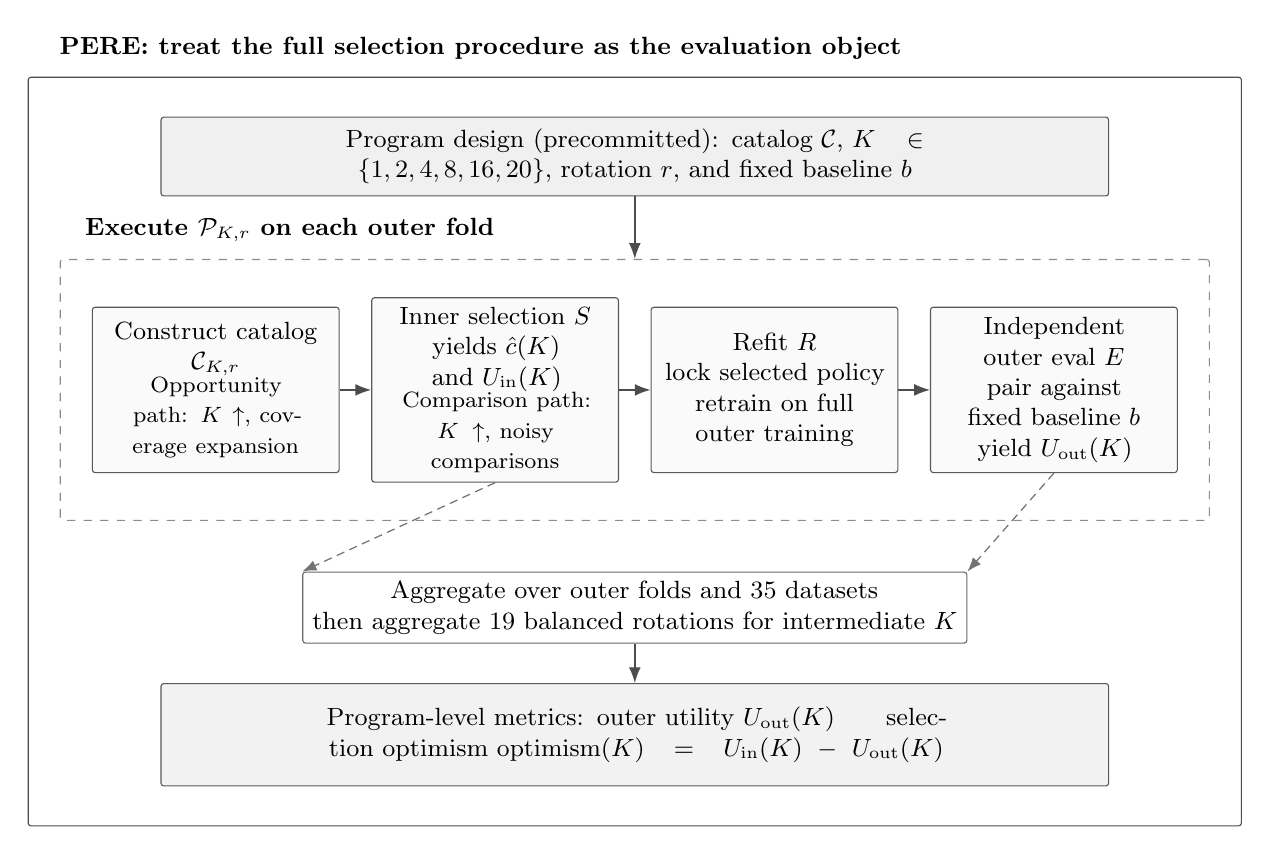
\begin{tikzpicture}[
  node distance=5mm and 4mm,
  stage/.style={draw=black!65, rounded corners=1pt, align=center, minimum height=21mm, text width=29mm, fill=black!2, font=\small},
  setting/.style={draw=black!65, rounded corners=1pt, align=center, minimum height=10mm, text width=118mm, fill=black!6, font=\small},
  aggregate/.style={draw=black!60, rounded corners=1pt, align=center, minimum height=9mm, text width=82mm, fill=white, font=\small},
  metric/.style={draw=black!65, rounded corners=1pt, align=center, minimum height=13mm, text width=118mm, fill=black!5, font=\small},
  arrow/.style={-{Latex[length=2mm]}, line width=0.5pt, draw=black!70},
  measure/.style={-{Latex[length=1.8mm]}, line width=0.45pt, draw=black!55, densely dashed}
]
\node[stage] (catalog) {Construct catalog\\$\mathcal{C}_{K,r}$\\[-1mm]{\footnotesize Opportunity path: $K\uparrow$, coverage expansion}};
\node[stage, right=of catalog] (select) {Inner selection $S$\\yields $\hat{c}(K)$ and $\uinner(K)$\\[-1mm]{\footnotesize Comparison path: $K\uparrow$, noisy comparisons}};
\node[stage, right=of select] (refit) {Refit $R$\\lock selected policy\\retrain on full outer training};
\node[stage, right=of refit] (outer) {Independent outer eval $E$\\pair against fixed baseline $b$\\yield $\uouter(K)$};
\draw[arrow] (catalog) -- (select);
\draw[arrow] (select) -- (refit);
\draw[arrow] (refit) -- (outer);
\node[draw=black!45, dashed, rounded corners=1pt, fit=(catalog)(outer), inner xsep=4mm, inner ysep=6mm] (program) {};
\node[font=\small\bfseries, anchor=south west] at ([xshift=2mm,yshift=1mm]program.north west) {Execute $\mathcal{P}_{K,r}$ on each outer fold};

\coordinate (programmid) at ($(catalog)!0.5!(outer)$);
\node[setting] (setting) at ([yshift=13mm]program.north) {Program design (precommitted): catalog $\mathcal{C}$, $K\in\{1,2,4,8,16,20\}$, rotation $r$, and fixed baseline $b$};
\draw[arrow] (setting.south) -- (program.north);

\node[aggregate] (aggregate) at ([yshift=-11mm]program.south) {Aggregate over outer folds and 35 datasets\\then aggregate 19 balanced rotations for intermediate $K$};
\draw[measure] (select.south) -- (aggregate.north west);
\draw[measure] (outer.south) -- (aggregate.north east);
\node[metric, below=5mm of aggregate] (metrics) {Program-level metrics: outer utility $\uouter(K)$\qquad selection optimism $\optm(K)=\uinner(K)-\uouter(K)$};
\draw[arrow] (aggregate) -- (metrics);

\node[draw=black!70, rounded corners=1pt, fit=(setting)(program)(metrics), inner xsep=4mm, inner ysep=5mm] (pere) {};
\node[font=\small\bfseries, fill=white, inner xsep=2mm, anchor=south west] at ([xshift=2mm,yshift=1mm]pere.north west) {PERE: treat the full selection procedure as the evaluation object};
\end{tikzpicture}
\caption{Overall problem definition of PERE. Predeclared design fixes the per-fold selection program $\mathcal P_{K,r}$; expanding $K$ introduces two paths --- ``coverage expansion'' at the catalog stage and ``noisy comparison increase'' at the inner selection stage. After aggregating outer-fold, rotation, and dataset-level results, the procedure reports outer utility and selection optimism jointly. Solid arrows mark program execution; dashed arrows mark metric sources.}
\label{fig:pere_definition}
\end{figure}

\subsection{A two-curve account of policy search}
Let $\mathcal{C}$ be a frozen catalog of candidate policies, each policy specifying a learner configuration and an augmentation component. Let $\mathcal{C}_K\subseteq\mathcal{C}$ be the scheduled pool of nominal size $K$. For candidate $c$, define $\delta_{\mathrm{in}}(c)$ as its paired inner out-of-fold AUC minus the corresponding baseline inner AUC. The selector chooses
\begin{equation}
 \hat c(K)=\arg\max_{c\in\mathcal{C}_K}\delta_{\mathrm{in}}(c).
\end{equation}
The apparent utility available at selection time is
\begin{equation}
 \uinner(K)=\delta_{\mathrm{in}}(\hat c(K)).
\end{equation}
After the selection is locked, the selected policy and baseline are refit on the outer-training data and measured on the untouched outer test fold. Their paired difference is $\uouter(K)$. Selection optimism is
\begin{equation}
 \optm(K)=\uinner(K)-\uouter(K).
\end{equation}
These are not alternative estimates of one quantity. They answer different questions. $\uinner(K)$ is the evidence that caused the selector to act; $\uouter(K)$ is the utility subsequently realized by that action; and $\optm(K)$ is the deployment gap created by selection and finite-sample estimation.

A larger $K$ can increase $\uouter$ because the selector gains access to a better policy. It can increase optimism because the maximum is taken over more noisy estimates. It can do both simultaneously. This is why statements such as ``search overfits'' or ``more search improves performance'' are incomplete. Search may produce positive deployment value while also making the winning inner score less credible. The operating decision depends on the joint curve.

\subsection{Why a knee is plausible but not universal}
Suppose early candidates add genuinely different inductive biases and later candidates mostly refine already represented behavior. Early pool expansions can then add outer utility rapidly. Once the main useful modes are represented, additional policies may still perturb the maximum inner estimate and win due partly to favorable noise, while adding little new outer value. The result is a knee: the outer curve bends toward a plateau before the optimism curve does.

Several mechanisms can produce this pattern. Candidate redundancy can make nominal growth exceed effective growth. Hyperparameter variants can differ in name but produce similar predictions. Augmentation can become a no-op in some folds, or its effect can be dominated by the learner. Finite dataset size can make small true differences hard to distinguish. A balanced schedule can also expose useful candidates early by design. Our data support the curve shape and document exact prediction duplication, but they do not identify one mechanism causally. Accordingly, ``knee around $K\approx8$'' means an observed diminishing-return region in this catalog and schedule. It does not mean that eight is a universal optimum or that a different ordering, catalog, corpus, or cost function would produce the same point.

\subsection{Deployment interpretation}
Treating $K$ as an operating specification changes what must be reported. A deployer should know the eligible policy catalog, the rule that maps training evidence to a selected policy, the nominal breadth searched, the validation boundary, and the fallback rule. Two systems that eventually choose random forest with no augmentation may still have different deployment difficulty if one selected it from four candidates and the other from twenty after extensive adaptive comparison. The named winner does not reveal the evidence exposure.

The same view clarifies that selection frequency is not a causal policy effect. A policy can be selected often because it is broadly competitive, because the schedule represents it in many useful pools, because its estimates are more variable, or because it interacts favorably with particular datasets. Frequency describes what the procedure does. It is valuable for deployment because it reveals whether the method is effectively fixed or genuinely adaptive, but it cannot establish that the most frequent learner is intrinsically superior.

\section{Study Design}
The study combines a supporting wide grid with a nested candidate search. The wide grid checks whether heterogeneous data genuinely require different learner--augmentation pairs; the nested search measures outer utility and selection optimism as the catalog expands. The two designs differ in catalog and validation protocol; their results are reported separately as complementary evidence.

Figure~\ref{fig:design} shows the nested pipeline used in the main experiment. The 20-policy catalog, the six $K$ values, and the subset construction rules are all precommitted; outer test outcomes are not consulted when these are set. Inner folds serve only to select; outer folds serve only to evaluate the realized utility of the locked procedure.

\begin{figure}[t]
\centering
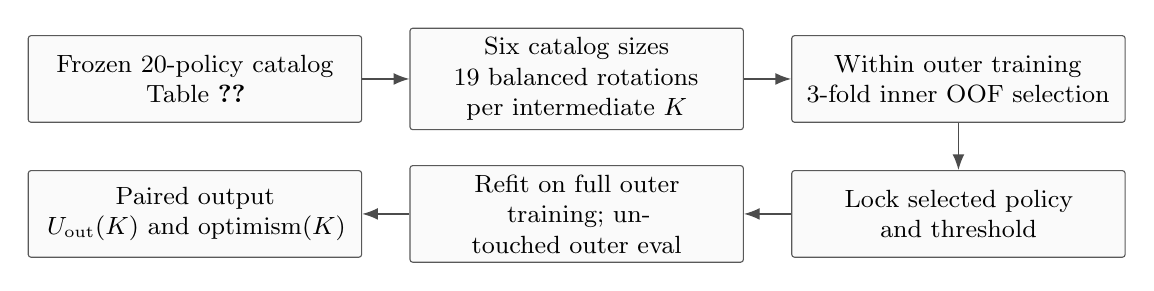
\begin{tikzpicture}[
  node distance=6mm and 6mm,
  box/.style={draw=black!65, rounded corners=1pt, align=center, minimum height=11mm, text width=40mm, fill=black!2, font=\small},
  arrow/.style={-{Latex[length=2mm]}, line width=0.5pt, draw=black!70}
]
\node[box] (catalog) {Frozen 20-policy catalog\\Table~\ref{tab:catalog}};
\node[box, right=of catalog] (schedule) {Six catalog sizes\\19 balanced rotations per intermediate $K$};
\node[box, right=of schedule] (inner) {Within outer training\\3-fold inner OOF selection};
\node[box, below=of inner] (lock) {Lock selected policy\\and threshold};
\node[box, left=of lock] (outer) {Refit on full outer\\training; untouched outer eval};
\node[box, left=of outer] (outputs) {Paired output\\$\uouter(K)$ and $\optm(K)$};
\draw[arrow] (catalog) -- (schedule);
\draw[arrow] (schedule) -- (inner);
\draw[arrow] (inner) -- (lock);
\draw[arrow] (lock) -- (outer);
\draw[arrow] (outer) -- (outputs);
\end{tikzpicture}
\caption{PERE nested evaluation pipeline for candidate search breadth. Candidate identities, six catalog sizes, and subset construction rules are precommitted; outer test labels do not participate in preprocessing, augmentation, candidate selection, or threshold determination.}
\label{fig:design}
\end{figure}

\subsection{Dataset corpus and inferential unit}
The corpus contains 35 datasets in six named benchmark families: AEEEM (5 datasets), JIRA (7), NASA (5), PROMISE (10), ReLink (3), and SOFTLAB (5). Dataset sizes range from 36 to 2,705 observations in the corrected descriptor artifact, with 20 to 65 features. Minority-class fractions range from approximately 0.074 to 0.495. These ranges are descriptive properties of this corpus, not claims about all SDP datasets.

The dataset is the independent inferential unit. Folds, outer seeds, fit repetitions, and intermediate-pool rotations are repeated measurements used to stabilize the dataset-level estimate. They are not treated as independent replications. This choice prevents precision from being inflated by counting correlated resamples as if they were new datasets. Family labels are used as bootstrap strata and for descriptive localization. Six observed families, including ReLink with only three datasets, do not support treating family means as six independently powered confirmations.

\begin{table}[t]
\caption{Study inventory. Family counts come from the RQ3 family summary; split and completion counts come from the final-summary artifacts.}
\label{tab:inventory}
\centering\small
\begin{tabular}{lr}
\toprule
Component & Declared value\\
\midrule
Datasets / families & 35 / 6\\
Family sizes & 5, 7, 5, 10, 3, 5\\
Canonical policy tuples & 20\\
Fixed baseline & \texttt{lr\_c1\_none}\\
Outer seeds / folds per seed & 3 / 5\\
Inner folds / fit repetitions & 3 / 3\\
Completed outer units & 525 / 525\\
Inferential unit & dataset ($N=35$)\\
Bootstrap draws & 10,000\\
\bottomrule
\end{tabular}
\end{table}

\subsection{Frozen policy catalog}
The corrected catalog contains 20 unique canonical tuples and includes the fixed baseline \texttt{lr\_c1\_none}. Candidate policies combine four learner families---logistic regression (LR), random forest (RF)~\cite{breiman2001rf}, XGBoost (XGB)~\cite{chen2016xgboost}, and multilayer perceptron (MLP)---with declared augmentation components drawn from none, SMOTE~\cite{chawla2002smote}, ADASYN~\cite{he2008adasyn}, and Borderline-SMOTE~\cite{han2005borderline}. Some learner families have multiple configurations. The catalog is a heterogeneous set of joint policies, not a factorial experiment designed to estimate separate learner and augmentation main effects. The full catalog is enumerated in Table~\ref{tab:catalog}.

\begin{table}[t]
\caption{Frozen 20-policy candidate catalog. A dash indicates no augmentation; \texttt{none} indicates unbounded tree depth. Table parameters vary across candidates; shared fixed items are listed in the main text.}
\label{tab:catalog}
\centering\fontsize{8pt}{9.5pt}\selectfont
\setlength{\tabcolsep}{3pt}
\begin{tabularx}{\textwidth}{@{}>{\raggedright\arraybackslash}p{50mm}l>{\raggedright\arraybackslash}Xl@{}}
\toprule
Candidate ID & Learner & Varying parameter & Augmentation\\
\midrule
\nolinkurl{lr_c0.1_none} & LR & $C=0.1$ & ---\\
\nolinkurl{lr_c1_none}$^{*}$ & LR & $C=1$ & ---\\
\nolinkurl{lr_c10_none} & LR & $C=10$ & ---\\
\nolinkurl{lr_c0.1_smote} & LR & $C=0.1$ & SMOTE\\
\nolinkurl{lr_c1_smote} & LR & $C=1$ & SMOTE\\
\nolinkurl{lr_c10_adasyn} & LR & $C=10$ & ADASYN\\
\nolinkurl{lr_c1_borderline_smote} & LR & $C=1$ & B-SMOTE\\
\nolinkurl{lr_c10_borderline_smote} & LR & $C=10$ & B-SMOTE\\
\nolinkurl{rf_n100_depthnone_none} & RF & $n=100,d=\texttt{none}$ & ---\\
\nolinkurl{rf_n100_depth10_smote} & RF & $n=100,d=10$ & SMOTE\\
\nolinkurl{rf_n300_depthnone_adasyn} & RF & $n=300,d=\texttt{none}$ & ADASYN\\
\nolinkurl{rf_n300_depth10_borderline_smote} & RF & $n=300,d=10$ & B-SMOTE\\
\nolinkurl{xgb_n100_depth3_none} & XGB & $n=100,d=3$ & ---\\
\nolinkurl{xgb_n100_depth6_smote} & XGB & $n=100,d=6$ & SMOTE\\
\nolinkurl{xgb_n300_depth3_adasyn} & XGB & $n=300,d=3$ & ADASYN\\
\nolinkurl{xgb_n300_depth6_borderline_smote} & XGB & $n=300,d=6$ & B-SMOTE\\
\nolinkurl{mlp_h32_alpha0.0001_none} & MLP & $h=32,\alpha=10^{-4}$ & ---\\
\nolinkurl{mlp_h32_alpha0.01_smote} & MLP & $h=32,\alpha=10^{-2}$ & SMOTE\\
\nolinkurl{mlp_h64_alpha0.0001_adasyn} & MLP & $h=64,\alpha=10^{-4}$ & ADASYN\\
\nolinkurl{mlp_h64_alpha0.01_borderline_smote} & MLP & $h=64,\alpha=10^{-2}$ & B-SMOTE\\
\bottomrule
\end{tabularx}
\vspace{1mm}
\parbox{0.97\textwidth}{\raggedright $^{*}$Fixed baseline. $n$ = number of trees or boosting rounds; $d$ = maximum depth; $h$ = single hidden-layer width; B-SMOTE = Borderline-SMOTE.}
\end{table}

This distinction is non-negotiable. The pool-size intervention changes access to candidate tuples. It does not vary the amount of synthetic data, the ratio of augmented to original observations, or an augmentation intensity. A policy with ``none'' can be selected at any breadth, and broader pools introduce learner and augmentation combinations together. Therefore the full-catalog outer gain cannot be attributed specifically to augmentation, and $K$ cannot be relabeled as an augmentation dose.

The baseline anchors both utility and harm. At $K=1$, only the baseline is available, so inner utility, outer utility, and optimism are defined as zero. At larger $K$, the selector may retain the baseline or choose another policy. This construction makes each curve a paired improvement over a fixed operational fallback rather than an absolute AUC curve whose level varies with dataset difficulty.

\subsection{Leakage-safe nested procedure}
For each dataset, the production design uses three outer split seeds and five outer folds per seed, yielding 15 outer units. Inside each outer-training partition, three inner folds produce out-of-fold predictions for selection. Stochastic candidate fitting is repeated three times. Preprocessing and augmentation are learned within the relevant training fold, so neither inner validation rows nor outer test rows are used to construct synthetic training data or fit transformations.

Candidate utility is computed as a paired difference from the fixed baseline on the same inner folds. The candidate with maximum mean paired inner OOF \dauc\ within the scheduled pool is recorded in a selection manifest. Only after this lock is the selected policy refit on the complete outer-training partition and evaluated on the untouched outer test partition. The baseline is refit and scored on that same partition, preserving pairing. For thresholded metrics, the selected policy and baseline receive separate thresholds derived from their own inner OOF predictions; no outer-test label is used to choose a threshold.

The complete Phase 2b run contains 525 of 525 expected outer units, 94,500 inner fits, and zero failures. These counts establish completion, not statistical sample size. The outer result estimates the behavior of the complete selection procedure under repeated nested splits. It is stronger than reporting the best test cell, but it remains internal benchmark evaluation rather than external validation on an independently collected corpus.

\subsection{Candidate-pool schedule}
Search breadth is evaluated at $K\in\{1,2,4,8,16,20\}$. The endpoints are fixed: $K=1$ is baseline-only and $K=20$ is the full catalog. Let $b$ denote the fixed baseline and order the 19 non-baseline candidates before any outer outcome is seen. Denote the resulting sequence by $M=(m_0,\ldots,m_{18})$. For $K\in\{2,4,8,16\}$ each intermediate size uses 19 rotations indexed $r\in\{0,\ldots,18\}$, and the per-fold candidate subset is
\begin{equation}
 \mathcal C_{K,r}=\{b\}\cup\{m_{(r+j)\bmod 19}:j=0,\ldots,K-2\}.
\end{equation}
At $K=1$ the only subset is $\{b\}$; at $K=20$ the only subset is the full catalog. The number of subsets per size is therefore $1,19,19,19,19,1$. Within a single rotation $r$ the subsets are strictly nested:
$\mathcal C_{1,r}\subset\mathcal C_{2,r}\subset\mathcal C_{4,r}\subset\mathcal C_{8,r}\subset\mathcal C_{16,r}\subset\mathcal C_{20,r}$.

For any intermediate $K$, every non-baseline candidate appears exactly $K-1$ times across the 19 rotations, so its marginal inclusion probability is $(K-1)/19$. The fixed baseline appears in every subset. The rotation balances inclusion counts only; it does not fix candidate co-occurrence or interactions. Across all six sizes the design yields 78 subsets in total.

Results are aggregated in four steps. Fit repetitions are averaged first; outer folds within each seed are averaged next; outer seeds are averaged next; and for intermediate sizes the 19 rotations are then averaged. The procedure leaves exactly one value per dataset, $K$, and metric. Grand-mean curves are then obtained by equal-weight averaging over the 35 datasets, so datasets with more observation rows do not receive higher weight.

For each dataset and $K$, aggregation first averages fit repetitions, then outer folds within seed, then outer seeds; intermediate rotations are also averaged for their scheduled pool sizes. The resulting artifact has one value per dataset per $K$ for each metric. Equal-weight means across the 35 datasets define the corpus-level curves. No large dataset receives greater inferential weight simply because it contains more rows.

\subsection{Outcomes and robustness metrics}
ROC-AUC is the primary performance measure because the selected-policy utility and pool-size analyses were predeclared around paired \dauc. At full catalog, we additionally report thresholded F1, G-measure, and Matthews correlation coefficient (MCC)~\cite{chicco2020mcc} under threshold 0.5 and under separately derived Youden thresholds~\cite{youden1950index}. These measures test whether the AUC direction is an artifact of ranking performance alone. They are robustness outcomes, not alternative endpoints selected after inspecting favorable results.

We also report an outer AUC harm rate: for each dataset, the fraction of its 15 outer units on which the selected policy underperforms the paired baseline in AUC. This is a process diagnostic. It complements the dataset-level mean by showing that a positive average can coexist with frequent local downside. It should not be interpreted as an independent binomial sample because outer units within a dataset are repeated split measurements.

\subsection{Exploratory routing descriptors}
The routing analysis uses four implemented statistics: label entropy, minority-class fraction, mean absolute off-diagonal feature correlation, and the fraction of highly correlated feature pairs. A signals-only model uses all four; an intrinsic-only model uses a smaller descriptor subset defined by the corrected analyzer. Standardized OLS fits summarize in-sample association. Leave-one-family-out (LOFO) ridge evaluation trains on five families and predicts the sixth, repeated over all six held-out families. An intercept-only predictor provides the relevant comparator.

This analysis is exploratory for three reasons. First, the 35 outcomes are the same repaired full-catalog outer values analyzed elsewhere, not an independent replication. Second, six family blocks provide little basis for complex routing inference. Third, only four coarse descriptors are tested. A failure to beat the intercept excludes a deployment claim for these descriptors; it does not prove that richer task embeddings, landmarkers, learning curves, or policy-interaction features cannot route.

\section{Analysis Plan}
\subsection{Primary and secondary estimands}
RQ1 reports the full-catalog dataset distribution of inner-selected \dauc, outer-realized \dauc, and optimism. Family-stratified percentile intervals use 10,000 bootstrap draws: datasets are resampled with replacement within each observed family, preserving family sample sizes, and the equal-weight dataset mean is recomputed. Direction counts are based on the 35 dataset aggregates.

RQ2's primary confirmatory estimand is the per-dataset OLS slope of optimism against $\log_2(K)$. A one-unit change corresponds to a doubling for the powers-of-two schedule; the final transition to $K=20$ remains represented at its actual log position. The 35 slopes are summarized by their mean and a family-stratified bootstrap interval, and tested against zero with a Wilcoxon signed-rank test. The key secondary estimand is the analogous outer \dauc\ slope.

Adjacent contrasts describe shape. Differences are formed within dataset for $2-1$, $4-2$, $8-4$, $16-8$, and $20-16$, then summarized across datasets. Wilcoxon tests are adjusted with Holm correction separately within the five optimism contrasts and the five outer-utility contrasts. For Figure~\ref{fig:marginal}, family-stratified bootstrap intervals for mean paired differences are reanalyzed directly from the corrected \texttt{dataset\_k\_summary.csv}. This adds uncertainty visualization but does not fit new predictive models or rerun any experiment.

\subsection{Heterogeneity and composition}
Dataset heterogeneity is shown by connecting each dataset's inner-selected and outer-realized \dauc\ at $K=20$. The connector length is its optimism. Family colors localize benchmark strata, while the zero line reveals negative outer outcomes. We report family means only as descriptive summaries and retain all raw dataset points to prevent a positive family mean from being mistaken for universal benefit.

Selected-policy composition is computed from the corrected candidate-frequency artifact. Each dataset contributes 15 full-catalog outer selections. We first aggregate candidate IDs into learner family and augmentation category within dataset, divide by the dataset's 15 selections, and only then average shares across datasets or families. This preserves the dataset as the descriptive unit. Exact aggregate counts over all 525 outer units are also reported because they answer a transparent process question---what the executed selector chose---but no confidence interval treats 525 units as independent.

\subsection{Claim boundaries}
All numerical claims use the designated analysis artifacts. The six family means are not interpreted as six confirmatory domain replications. Prediction-hash duplication is used only as a diagnostic consistent with effective redundancy. The old augmentation-intensity claim is excluded.

\section{Results}

\subsection{Supporting wide grid: descriptive optima vary across datasets}
The supporting wide grid was run before the nested main experiment in order to test whether heterogeneous SDP data genuinely require different learner--augmentation pairs. Of the 12{,}150 comparison cells in that grid, 12{,}120 produced valid outcomes (99.75\%). The remaining 30 cells come from the ReLink Apache / ADASYN combination, spanning 10 classifiers and 3 seeds; the other 44 datasets had all 90 combinations available, and ReLink Apache had 80 usable combinations. Table~\ref{tab:broadgrid} summarizes dataset-internal comparisons after seed averaging.

\begin{table}[t]
\caption{Descriptive outcomes of the supporting wide grid. The AUC span is the maximum seed-averaged AUC minus the minimum across the available combinations on each dataset.}
\label{tab:broadgrid}
\centering\small
\setlength{\tabcolsep}{3.5pt}
\begin{tabular}{lrrrrr}
\toprule
Scope & Valid cells & Optima & Mean & Median & Maximum\\
\midrule
All 45 datasets & 12{,}120 & 29 & 0.327 & 0.320 & 0.669\\
Overlapping 35 datasets & 9{,}420 & 25 & 0.362 & 0.358 & 0.669\\
\bottomrule
\end{tabular}
\end{table}

Across the 45 datasets the AUC span has mean 0.327, median 0.320, and maximum 0.669. Twenty-nine distinct descriptive optima appear across datasets; no single combination dominates a majority of them. LightGBM-family classifiers appear in 12 of 45 dataset optima, the highest classifier frequency; by processing component, no-augmentation and KCO each appear in 8 of 45 datasets, tied for highest. The remaining optima are distributed across different resampling, filtering, cost-sensitive, and transfer combinations.

The 35 static datasets that overlap with the nested main experiment still show 25 distinct descriptive optima, with a mean AUC span of 0.362, indicating that candidate heterogeneity is not driven solely by the additional JIT datasets. JIT data is also included in the wide grid, but only to test whether candidate behavior varies with the observational unit. The maximum AUC values in the table are post-hoc statistics obtained after viewing all results on a dataset; the wide grid characterizes how candidate behavior varies across datasets, while the outer-fold gain of the selector is reported by the nested candidate-search results in RQ1--RQ4 below.

\subsection{RQ1: full-catalog selection realizes positive held-out value}
At $K=20$, mean inner-selected utility is $+0.0568$ \dauc\ (median $+0.0472$, family-stratified 95\% interval $[+0.0483,+0.0660]$). The corresponding mean outer-realized utility is $+0.0279$ (median $+0.0239$, interval $[+0.0166,+0.0399]$). Twenty-nine of 35 dataset aggregates are positive and six are negative. Thus the adaptive procedure delivers positive mean held-out value over the fixed baseline in this corpus, and the interval on that mean excludes zero.

The value claim attaches to the selector, not to a retrospective champion. The policy is chosen separately inside each outer unit, so the result measures what happens when the declared procedure receives training data, compares eligible policies using inner evidence, and deploys the selected pipeline. It does not establish that one named learner should replace the baseline on every dataset. Indeed, the composition analysis below shows that the roster varies substantially.

Mean full-catalog optimism is $+0.0289$ \dauc\ (median $+0.0227$, interval $[+0.0217,+0.0357]$), with 32 positive and three negative dataset values. The apparent inner gain is therefore about twice the realized outer gain in absolute terms: $0.0568$ versus $0.0279$. That comparison is not a ratio estimand and should not be read as a fixed shrinkage factor. It does show that reporting the selected inner score as expected deployment improvement would materially overstate the observed held-out utility.

Thresholded robustness outcomes are directionally consistent. At threshold 0.5, mean outer differences are $+0.0734$ for F1, $+0.0991$ for G-measure, and $+0.0475$ for MCC. Under separately derived Youden thresholds they are $+0.0263$, $+0.0276$, and $+0.0322$, respectively. The smaller Youden improvements are plausible because the baseline and selected policy each receive an inner-derived operating threshold, reducing the advantage that can arise when a fixed threshold is poorly calibrated for one method. These outcomes support a broad selected-pipeline benefit but do not replace AUC as the primary search-breadth estimand.

\begin{table}[t]
\caption{High-value full-catalog outcome summary. Intervals are 10,000-draw family-stratified percentile intervals over 35 dataset aggregates, from \texttt{rq5\_outcome\_summary.csv}.}
\label{tab:outcomes}
\centering\small
\begin{tabular}{lrrr}
\toprule
Outcome & Mean & Median & 95\% interval\\
\midrule
Inner $\Delta$AUC & 0.0568 & 0.0472 & [0.0483,0.0660]\\
Outer $\Delta$AUC & 0.0279 & 0.0239 & [0.0166,0.0399]\\
Optimism & 0.0289 & 0.0227 & [0.0217,0.0357]\\
F1 ($t=0.5$) & 0.0734 & 0.0707 & [0.0488,0.0986]\\
G ($t=0.5$) & 0.0991 & 0.0846 & [0.0700,0.1282]\\
MCC ($t=0.5$) & 0.0475 & 0.0402 & [0.0266,0.0689]\\
\bottomrule
\end{tabular}
\end{table}

\subsection{RQ2: paired curves make the search trade-off visible}
Figure~\ref{fig:curves} is the paper's central result. At $K=1$, the baseline is the only eligible policy, so both curves begin at zero. Mean outer \dauc\ then rises to $+0.0093$, $+0.0199$, $+0.0261$, $+0.0274$, and $+0.0279$ at $K=2,4,8,16,20$. Mean optimism rises to $+0.0106$, $+0.0183$, $+0.0243$, $+0.0281$, and $+0.0289$. The faint trajectories show the 35 dataset-level paths, while the solid lines and shaded bands show equal-weight means and family-stratified intervals.

\begin{figure*}[t]
\centering
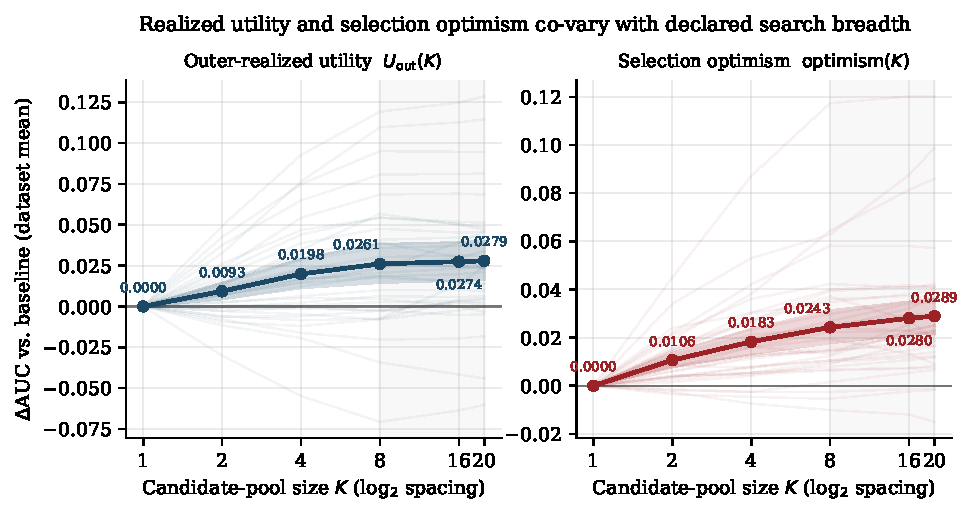
\includegraphics[width=0.74\textwidth]{fig3_paired_k_curves.pdf}
\caption{Paired outer-realized-utility and selection-optimism curves over the precommitted pool schedule. Solid points are equal-weight means over 35 dataset aggregates; bands are family-stratified 95\% bootstrap intervals; faint lines are dataset trajectories. Values come from \texttt{pool\_summary.csv} and \texttt{dataset\_k\_summary.csv}. The shaded late region marks $K\geq8$ for visual orientation, not a fitted change point.}
\label{fig:curves}
\end{figure*}

The optimism slope is $+0.0065$ per unit of $\log_2(K)$, with interval $[+0.0049,+0.0081]$ and Wilcoxon $p=5.12\times10^{-9}$. This is the primary confirmatory result: within the frozen catalog and balanced schedule, datasets tend to show a larger inner-to-outer gap as nominal search opportunity expands. The outer-utility slope is also positive, $+0.0065$ per log-two unit, with interval $[+0.0039,+0.0092]$ and $p=2.87\times10^{-5}$. Broader search therefore creates real mean value as well as optimism.

The two slopes round to the same value, but this numerical equality should not be overinterpreted. They are calculated from different dataset-level quantities and answer different questions. Their curve shapes provide the operational information that the rounded slopes conceal. The outer curve rises quickly through $K=8$ and then changes little, whereas the optimism curve continues to rise through every expansion. A single linear slope is useful for confirming direction; it is insufficient for choosing or reporting an operating region.

\subsection{RQ2 marginal returns and heterogeneous realization}
Figure~\ref{fig:marginal} shows paired adjacent increments. Outer utility increases by $+0.0093$ from $K=1$ to 2, $+0.0106$ from 2 to 4, and $+0.0062$ from 4 to 8. All three are positive after Holm correction. The final increments are $+0.0013$ from 8 to 16 and $+0.0005$ from 16 to 20; both have Holm-adjusted $p=0.771$. The absence of significance does not prove exact equality, but the effect estimates and intervals show that late gains are small relative to early gains.

\begin{figure*}[t]
\centering
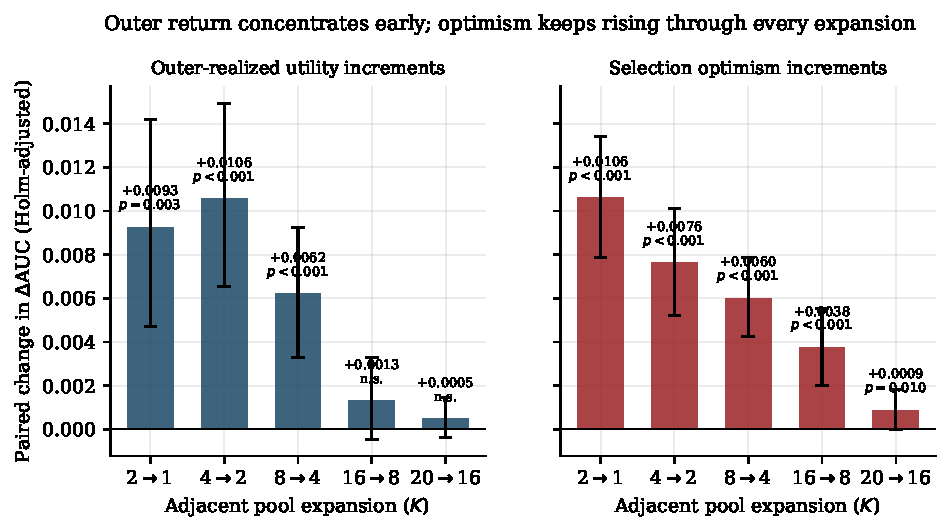
\includegraphics[width=0.74\textwidth]{fig4_marginal_knee.pdf}
\caption{Within-dataset adjacent changes in outer-realized utility and optimism. Bars are mean paired differences over 35 datasets; error bars are family-stratified 95\% bootstrap intervals reanalyzed from corrected \texttt{dataset\_k\_summary.csv}; annotations report corrected means and Holm-adjusted Wilcoxon results from \texttt{adjacent\_contrasts.csv}. The last two outer increments are not distinguishable from zero, whereas every optimism increment is positive after adjustment.}
\label{fig:marginal}
\end{figure*}

By $K=8$, mean outer utility is $0.0261/0.0279=93.5\%$ of the full-catalog mean. By $K=16$, it is 98.2\%. These percentages summarize observed acquisition in this schedule; they are not probabilities and do not estimate the best $K$ for a future catalog. They nevertheless make the practical shape concrete. Moving from one to eight candidates captures most observed mean benefit. Searching the final twelve nominal candidates adds $+0.0018$ mean outer \dauc\ while optimism grows by $+0.0046$ over the same region.

Optimism increments are $+0.0106$, $+0.0077$, $+0.0060$, $+0.0038$, and $+0.0008$. All five remain Holm-significant, including $K=20$ versus 16 with adjusted $p=0.0101$. The increments themselves shrink, so optimism also approaches saturation, but it does so more slowly and remains detectably responsive after the outer curve has flattened. This pattern is the empirical basis for treating search breadth as a deployment-difficulty parameter: late search continues to alter the credibility gap even when its measurable realized return is limited.

The knee should be understood as an operating region rather than an optimum. We did not assign monetary costs to model fits, errors, or search latency; nor did we fit a change-point model. A deployment with very high error cost might value even a small mean outer increment, while a resource-constrained deployment might prefer a smaller catalog. The supported statement is narrower: in this catalog, outer gains are concentrated through approximately $K=8$, and the final expansions add little distinguishable mean outer value while optimism continues to accumulate.

The grand means can suggest a simple story in which every dataset gains about 0.028 AUC and loses another 0.029 to optimism. Figure~\ref{fig:datasets} rejects that simplification. Full-catalog outer values range from $-0.0603$ for SOFTLAB AR6 to $+0.1286$ for ReLink ZXing. The six negative aggregates are SOFTLAB AR5 and AR6, ReLink Apache, PROMISE Velocity and Ivy, and JIRA JRuby. The negative Ivy value is close to zero, whereas AR5 and AR6 show material downside.

\begin{figure*}[t]
\centering
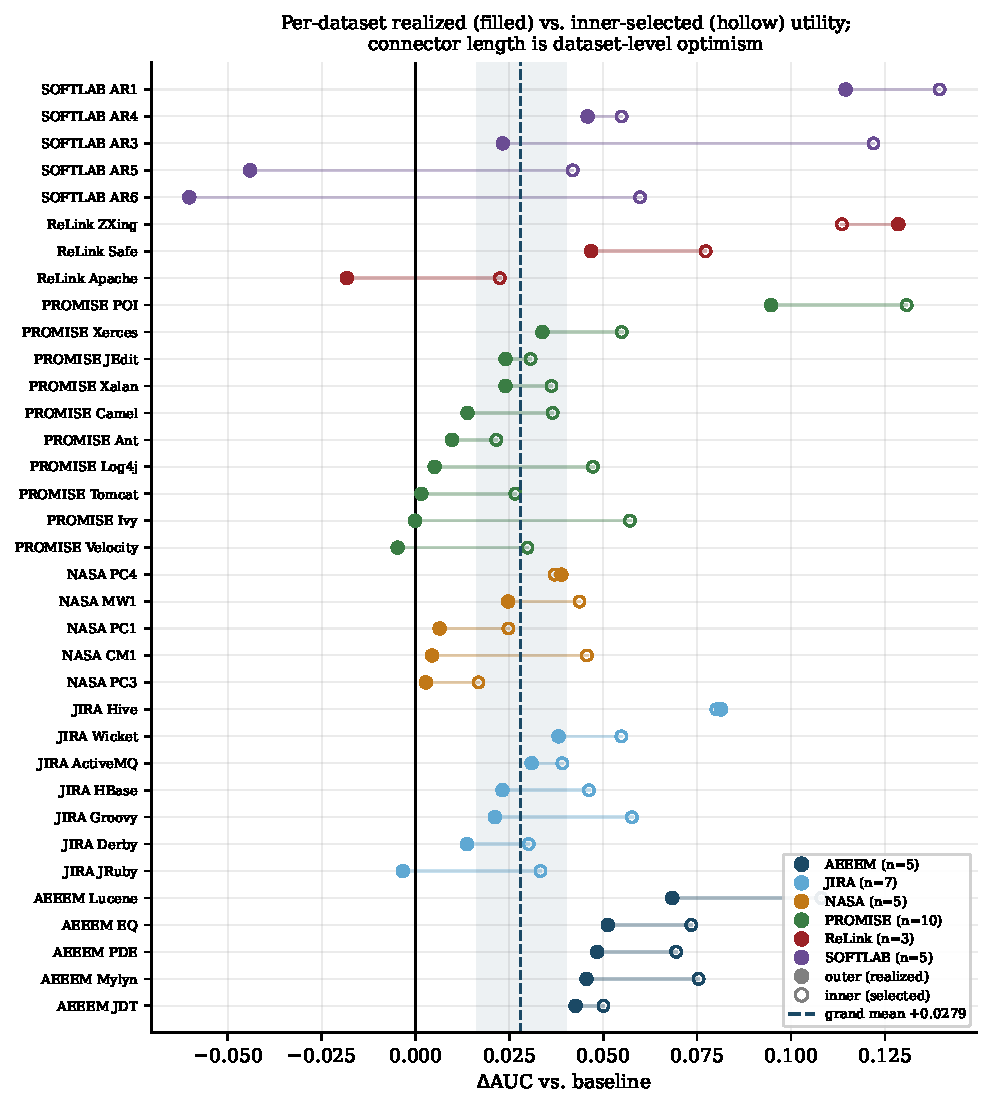
\includegraphics[width=0.68\textwidth]{fig5_dataset_heterogeneity.pdf}
\caption{Dataset-level full-catalog utility. Filled points are outer-realized \dauc; hollow points are inner-selected \dauc; connectors are dataset-level optimism. Datasets are grouped by family and sorted within family by outer utility. The dashed line and band are the overall outer mean and family-stratified 95\% interval. Values come directly from corrected \texttt{rq5\_dataset\_values.csv}; no fold-level uncertainty is shown because the inferential unit is the dataset.}
\label{fig:datasets}
\end{figure*}

The connector lengths also vary. SOFTLAB AR6 has inner-selected utility $+0.0598$ but outer utility $-0.0603$, producing optimism $+0.1201$, the largest in the corpus. ReLink ZXing lies at the opposite extreme: inner-selected utility is $+0.1136$ and outer utility is even larger at $+0.1286$, producing slightly negative optimism. JIRA Hive also has negative optimism because its outer gain exceeds its inner estimate. These cases illustrate why optimism is a dataset-level random quantity, not a deterministic penalty subtracted from every selected score.

For deployment, the heterogeneity has two implications. First, a positive corpus mean does not guarantee benefit on a new dataset. A selector can be valuable on average while harming a nontrivial subset. Second, observing high inner gain is not sufficient to identify which datasets will realize it. AR6 appears promising inside and performs poorly outside; ZXing realizes more than its inner estimate. Deployment risk therefore requires the outer distribution and fallback behavior, not merely a corrected grand mean.

\subsection{Family summaries localize variation but do not create six replications}
All six family means are positive at $K=20$: AEEEM $+0.0512$, JIRA $+0.0293$, NASA $+0.0154$, PROMISE $+0.0202$, ReLink $+0.0524$, and SOFTLAB $+0.0159$. This breadth is useful because the overall result is not produced by one negative family being overwhelmed by another large positive family. It is not evidence of uniformity. Figure~\ref{fig:families} overlays raw dataset values and shows that ReLink and SOFTLAB have especially wide within-family ranges.

\begin{figure*}[t]
\centering
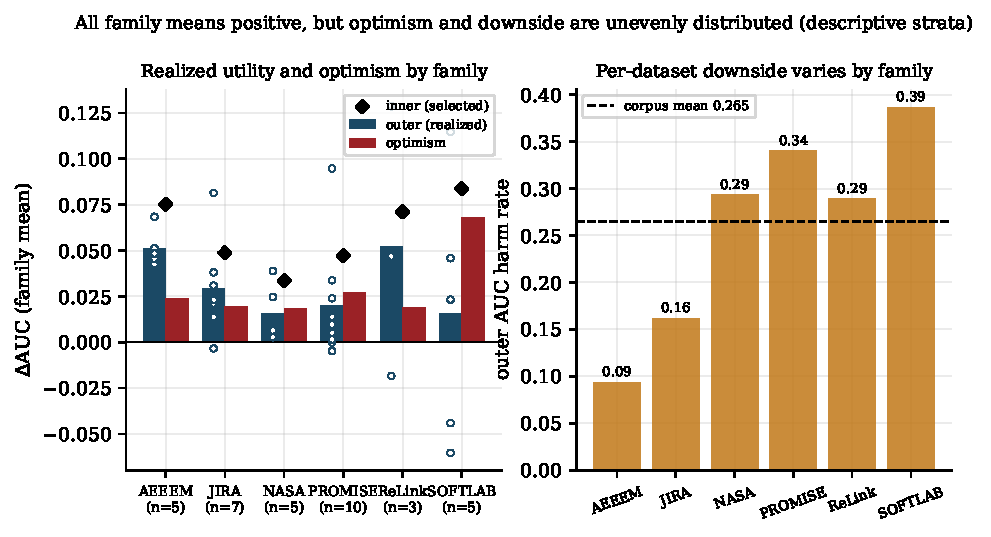
\includegraphics[width=0.74\textwidth]{fig6_family_summary.pdf}
\caption{Descriptive family localization at full catalog. Left: family means of outer utility and optimism, with inner-selected utility as diamonds and raw dataset outer values overlaid. Right: mean outer AUC harm rate by family. Values come from corrected \texttt{rq5\_family\_summary.csv} and \texttt{rq5\_dataset\_values.csv}. Family summaries are descriptive strata; ReLink has $n=3$, and the six means are not treated as independent confirmatory replications.}
\label{fig:families}
\end{figure*}

AEEEM combines the largest stable family mean among the better-populated families with the lowest mean harm rate, 0.0933. SOFTLAB has a similar mean inner-selected gain to AEEEM but a much smaller outer mean and the highest optimism, $+0.0678$, because AR5 and AR6 fail sharply outside. Its mean harm rate is 0.3867. PROMISE has a modest positive outer mean but harm rate 0.3400. NASA's outer mean is $+0.0154$ with harm rate 0.2933. JIRA is more favorable at $+0.0293$ outer and 0.1619 harm rate. ReLink's high mean outer utility is driven by only three datasets that span $-0.0183$ to $+0.1286$; interpreting that mean as a stable family effect would be unwarranted.

Family structure therefore helps explain where deployment risk is concentrated, but the raw dataset distribution remains primary. Positive family means can coexist with harmful datasets in four families. A deployment report that lists only the grand mean or even only six family means would hide the units on which the selected procedure fails.

\subsection{RQ3: policy composition shows genuine adaptivity}
The full-catalog selector does not collapse to one champion. Across 525 outer units, RF policies are selected 275 times (52.4\%), XGB 132 times (25.1\%), LR 100 times (19.0\%), and MLP 18 times (3.4\%). By augmentation component, no augmentation is selected 219 times (41.7\%), Borderline-SMOTE 112 (21.3\%), ADASYN 103 (19.6\%), and SMOTE 91 (17.3\%). The fixed baseline itself is selected in only 6 of 525 units (1.14\%) and appears at least once in six datasets.

\begin{figure*}[t]
\centering
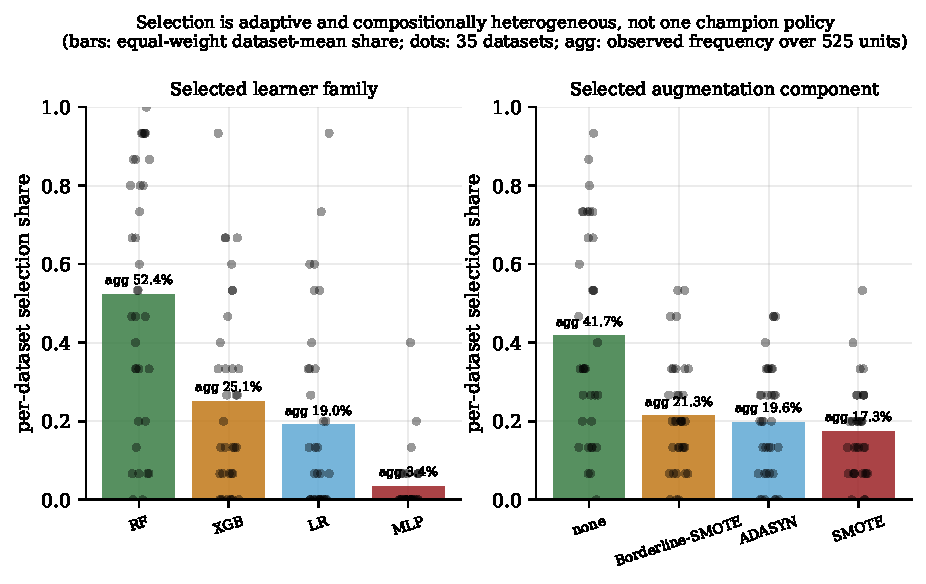
\includegraphics[width=0.74\textwidth]{fig7_selected_composition.pdf}
\caption{Composition of selected full-catalog policies. Bars are equal-weight means of per-dataset selection shares; dots are the 35 dataset shares, each computed from 15 outer units; annotations give exact aggregate frequencies across the 525 executed selections. Candidate IDs are grouped into learner family and augmentation component using \texttt{rq5\_selected\_candidate\_frequency.csv}. Frequencies describe the selector's behavior and are not causal estimates of learner or augmentation superiority.}
\label{fig:composition}
\end{figure*}

RF's aggregate majority does not mean that the study establishes RF as the best SDP learner. Dataset-level shares range from zero to one, and some datasets favor XGB or LR frequently. Selection frequency is shaped by the catalog's configurations, the inner evidence, candidate variance, and dataset interactions. A learner represented by several competitive tuples also has more ways to be selected than a single fixed policy. The correct conclusion is that the procedure uses heterogeneous choices and that its positive outer mean is not merely the performance of one hidden fixed model.

The augmentation panel has a similarly bounded interpretation. ``None'' is the largest single category, yet augmentation-bearing policies constitute 58.3\% of selections in aggregate. All four categories have substantial dataset-to-dataset spread. This is evidence that the selector sometimes uses augmentation and sometimes does not. It is not a factorial contrast of augmentation methods, because learners, hyperparameters, and augmentation components vary jointly and candidates were selected adaptively. In particular, the pool-size curve must not be interpreted as showing that more augmentation improves performance.

Composition matters for deployment in three ways. First, the full procedure requires maintaining multiple learner and preprocessing implementations; reporting only the most common family understates operational complexity. Second, a fallback policy remains necessary because selection can produce downside even when an advanced policy wins inner comparison. Third, compacting the catalog should preserve useful composition rather than simply retaining the globally most frequent candidates. A candidate selected rarely overall may be essential for a small subset of datasets.

\subsection{RQ4: exploratory routing analysis}
The signals-only descriptive fit has $R^2=0.1343$, RMSE $0.0354$, and MAE $0.0263$, compared with intrinsic-only $R^2=0.0374$, RMSE $0.0373$, and MAE $0.0271$. In sample, the four measured signals explain more variation. This apparent advantage disappears under the relevant generalization test. LOFO MAE is $0.0335$ for signals-only and $0.0339$ for intrinsic-only, both worse than the intercept-only comparator at $0.0294$.

\begin{figure*}[t]
\centering
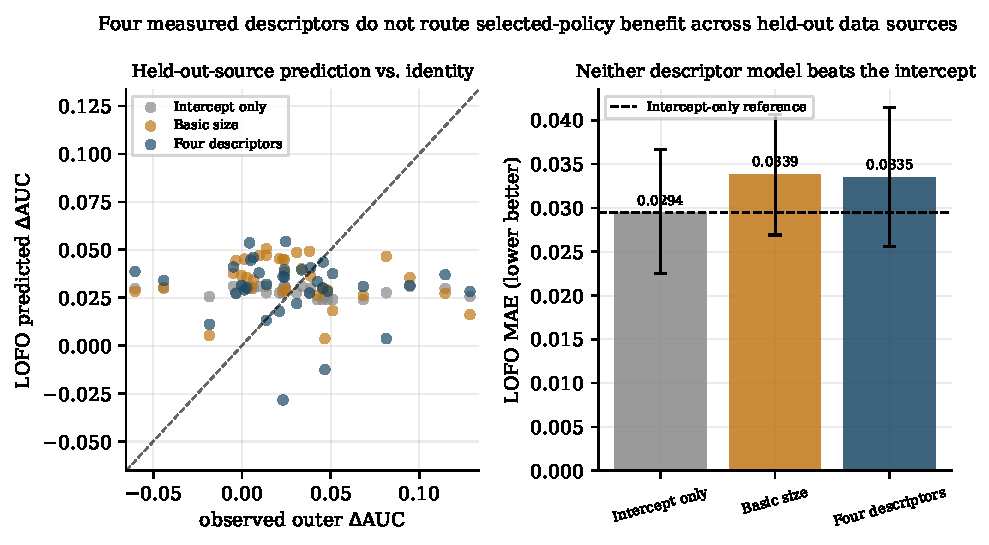
\includegraphics[width=0.74\textwidth]{fig8_routing_null.pdf}
\caption{Exploratory cross-family routing boundary. Left: leave-one-family-out predicted versus observed outer \dauc\ for intercept-only, intrinsic-only, and signals-only models. Right: LOFO MAE with family-stratified bootstrap intervals. Sources are \texttt{rq5\_lofo\_predictions.csv}, \texttt{rq5\_lofo\_summary.csv}, and \texttt{rq5\_model\_fit.csv}. Lower MAE is better; neither descriptor model improves on the intercept.}
\label{fig:routing}
\end{figure*}

The prediction scatter explains the null. Descriptor models compress predictions toward a modest positive range and fail to track large positive and negative dataset outcomes. With only six held-out family blocks, the analysis cannot support fine-grained inference about which descriptor fails. The bounded conclusion is practical: these four statistics do not provide a deployment-ready router for selected-policy benefit in this corpus. A system cannot currently use them to justify replacing the measured $K$ schedule with a smaller predicted subset.

This negative result strengthens the operating-specification argument. If a validated router existed, search breadth could be conditional on dataset characteristics. In its absence, the declared catalog and $K$ remain observable properties of the deployed selection procedure. Future routers should be evaluated in an additional outer layer, because learning which candidates to search is itself adaptive model selection.

\section{Discussion}
\subsection{Search can be valuable and optimistic at the same time}
The main finding resists a common binary framing. Broader search is neither simply beneficial nor simply overfitting. In the tested catalog it delivers positive outer value and increases optimism. The full selector improves mean outer AUC by $+0.0279$, but its mean inner-selected gain is $+0.0568$. Treating the inner score as the expected benefit would exaggerate deployment value; rejecting search because it creates optimism would discard a real positive outer gain. Sound deployment selection requires reporting both.

The paired curves make this duality operational. Early expansions add candidates that, on average, improve the selected outer pipeline. They also increase the maximization opportunity that separates selected inner evidence from outer realization. By $K=8$, most full-catalog utility is already present. Later expansions add little distinguishable mean outer value but continue to widen the deployment gap. This is exactly the information hidden when a paper reports only the final winning score or only the full search space.

The result also clarifies the role of nested evaluation. Nested CV is not merely a conservative correction that lowers a headline number. It estimates a different object: the performance of the selection algorithm after its adaptive choice. The gap between $\uinner$ and $\uouter$ is scientifically meaningful because it characterizes how much confidence should be placed in the selected evidence at a declared search breadth.

\subsection{Interpreting the knee without declaring an optimum}
The observed knee around $K\approx8$ offers guidance but not a universal prescription. Outer mean utility reaches 93.5\% of its full-catalog value by eight candidates, and neither subsequent adjacent gain is significant after Holm correction. A compact operating region near 8--16 candidates is therefore empirically plausible for this catalog. Choosing within that region, however, depends on deployment costs, acceptable downside, candidate fit costs, and the value assigned to small performance increments.

We deliberately avoid ``$K=8$ is optimal.'' An optimum requires an objective function. Candidate count ignores unequal compute and engineering cost. The schedule uses balanced rotations rather than one fixed production ordering. A different catalog could place a uniquely useful policy at position 20. A larger external corpus could distinguish a small late gain that 35 datasets cannot. The paper supports an empirical diminishing-return region, not a transportable constant.

A more mature operating specification would report both nominal breadth and effective breadth. Exact prediction hashes show 14,675 distinct hashes, 1,061 duplicate groups, and 3,183 records in duplicate groups in the routing diagnostic. This proves that nominally different candidate records can produce identical outer predictions. It does not measure near-duplicate errors, calibration differences, or causal contribution to the plateau. Still, it motivates a next study that manipulates candidate count and behavioral diversity separately. The diversity literature suggests that useful opportunity depends on error structure rather than count alone \cite{osei2025diversity}.

\subsection{Heterogeneity changes the deployment claim}
The positive mean is broad but not universal. All family means are positive, yet six datasets have negative aggregates and four families contain at least one negative dataset. The range from $-0.0603$ to $+0.1286$ is much larger than the grand mean. Some of the largest inner gains correspond to large optimism rather than large outer value. Consequently, deployment should not be justified by the corpus mean alone.

A practical selector needs a fallback and monitoring rule. The fixed baseline provides one natural reference. If inner evidence is weak, unstable, or inconsistent across folds, the system could retain the baseline rather than force a nonbaseline choice, although such a rule would need separate predefinition and evaluation. After deployment, monitoring should focus on calibration, ranking stability, and changes in data distribution rather than assuming that a catalog-level average guarantees local benefit.

Family summaries can guide hypothesis formation. AEEEM appears comparatively stable; SOFTLAB combines high inner opportunity with high optimism and harm. But the family counts are too small to support family-specific prescriptions. ReLink's mean, for example, averages only three sharply different datasets. The appropriate use of family structure is descriptive localization and stratified resampling, not six-domain generalization claims.

\subsection{What broader search changes inside the selector}
Broader search changes both the opportunity set and the statistical contest. Early additions can introduce behavior absent from a baseline-only pool and account for the observed outer gains through the early schedule Later additions can still win inner comparisons through favorable finite-sample error while adding little measured outer value. Thus the plateau concerns this catalog and balanced schedule, not a universal candidate count.

A compact deployment needs a frozen subset-selection rule and an independent assessment layer. Candidate frequency, fit cost, behavioral diversity, and failure robustness may inform that rule, but selecting a subset using the same outer outcomes would add another adaptive layer. Larger catalogs also increase implementation and maintenance exposure, which reinforces the need to report breadth explicitly.

\subsection{Wide grid and nested results answer different questions}
The supporting wide grid first motivates why candidate search is needed at all. Across 45 datasets, 29 distinct descriptive optima appear; on the 35 static datasets that overlap with the nested main experiment, 25 optima still appear, with substantial dataset-internal AUC spans. A single fixed combination is therefore unlikely to cover all datasets, and a candidate catalog has to accommodate different learners and processing components.

Candidate heterogeneity and search utility are two successive questions. The wide-grid optima are identified after viewing all plain cross-validation outcomes; they answer \emph{which combinations look different in hindsight}. The nested experiment, by contrast, requires the selector to decide before the outer outcomes are visible; it answers \emph{how much outer value is actually realized after searching}. The two layers of evidence jointly show that candidate heterogeneity provides an opportunity space for search, while nested evaluation quantifies how much of that space is redeemed in held-out data.

The candidate scope also differs across the two layers. The wide grid includes LightGBM, cost-sensitive, and CORAL variants, whereas the nested catalog substitutes XGBoost for some of those policies and freezes the search space into 20 canonical tuples. The wide grid characterizes candidate heterogeneity; the nested experiment provides the outer-utility curve within the 20-policy catalog. The 90 wide-grid combinations correspond to a different search space, and their diminishing-return behavior would have to be measured by a separate nested design.

\subsection{Negative outer results and baseline retention}
Although all six family means are positive, 6 of 35 datasets still have negative outer aggregates, and four of the six families contain at least one negative dataset, with dataset-level outcomes ranging from $-0.0603$ to $+0.1286$. Some of the largest inner gains correspond to large optimism rather than large outer value. The grand mean describes the average behavior of the selector; the dataset-level distribution reveals where the selector does and does not apply.

On some datasets, inner-evidence-driven selection produces negative outer utility, and inner evidence becomes detached from outer performance. One natural response is to specify a fallback rule: retain the baseline when inner evidence is unstable. The present study isolates the candidate-pool-size intervention, so concrete baseline-retention rules are left for separate evaluation; any such rule must be pre-specified and then tested on independent data. In practice, calibration, ranking stability, and data-distribution shifts also need continuous monitoring after deployment.

The contrast between SOFTLAB and ReLink illustrates the gap concretely. SOFTLAB AR5 reaches an inner gain of $+0.066$, but its outer utility is negative, and AR6 is negative as well; the family-level mean harm rate is 0.39. If selection conclusions were drawn from inner scores alone, this downside would be systematically underestimated. ReLink, by contrast, contains three datasets whose outer utilities span $-0.018$ to $+0.129$, with a family mean of $+0.052$ and large within-family dispersion. For both families, baseline retention and monitoring rules therefore need to be pre-evaluated rather than derived from a single average.

\subsection{Future work: extending the search object}
The present study isolates the candidate-pool-size intervention over a fixed joint learner-and-resampling search object. A natural next step is to include fold-internal feature selection inside the candidate pipeline and to evaluate it on outer folds that were not consulted during selection, so that the outer utility and selection optimism of feature-subset search can be compared with those of modeling-policy search. This would extend the selection-procedure evaluation in this paper toward a fuller feature-and-model joint search.

\section{Threats to Validity and Protocol Boundaries}
\subsection{Internal and statistical validity}
Selection is restricted to inner folds, preprocessing and augmentation are fold local, and outer labels are downstream of the selection lock. Completion is 525/525 outer units with zero recorded failures. These properties support an interpretation of outer \dauc\ as the performance of the selection procedure. They do not eliminate all implementation risk. The claim manifest and deterministic reproduction audit reduce that risk by tracing every reported value to machine-readable corrected artifacts.

Inference uses 35 dataset aggregates. Repeated seeds, folds, fit repetitions, and rotations stabilize estimates but are not independent observations. Family-stratified bootstrap intervals preserve observed family counts, yet only six strata exist and ReLink has three datasets. The intervals characterize this corpus under the stated resampling scheme; they are not population guarantees for all SDP projects. Adjacent tests describe five predeclared contrasts and use Holm adjustment within outcome families.

\subsection{Construct validity}
$K$ measures nominal candidate-pool breadth. It is not wall-clock budget, energy cost, augmentation intensity, or effective predictive diversity. Candidates differ in training cost and can behave redundantly. The late plateau may reflect redundancy, weak additions, ordering, finite power, or interactions among these factors. Prediction-hash duplication is diagnostic evidence of exact behavioral overlap, not a causal diversity analysis.

ROC-AUC is the primary outcome and does not encode a deployment threshold or defect-review cost. F1, G-measure, and MCC robustness summaries are positive under fixed and separately derived thresholds, but no cost-sensitive utility function is estimated. The operating recommendation should therefore be combined with project-specific costs before deployment.

\subsection{External validity}
The corpus contains 35 established benchmark datasets in six families. It does not include independently collected contemporary industrial streams, temporal deployment shifts, or all forms of software metrics. Untouched outer folds provide internal prospective evaluation within each dataset; they are not independent external validation. The magnitude and location of the knee may change with other catalogs, families, ordering rules, or learners.

The routing null is limited to four descriptors and six family blocks. It does not exclude richer meta-learning or pre-hoc recommendation. Recent work itself finds that global meta-feature explanations can be fragile \cite{herre2026metafeatures}, but this convergence does not establish a general impossibility theorem.

\section{Conclusion}
Search breadth is not an incidental implementation detail in software defect prediction. It defines both the opportunity available to a policy selector and the amount of noisy evidence over which the selector can optimize. In a frozen 20-policy catalog evaluated with inner-only selection and untouched outer folds, broader search delivered positive mean held-out utility while accumulating selection optimism. Mean outer \dauc\ reached $+0.0279$ at full catalog, with 29 of 35 dataset aggregates positive, but the corresponding inner-selected gain was $+0.0568$ and optimism was $+0.0289$.

The paired $K$ curves provide the substantive result: outer return was concentrated through approximately $K=8$, reaching 93.5\% of the full-catalog mean, while optimism increased at every expansion and the final two outer increments were not distinguishable from zero. Dataset and family analyses show that this average masks meaningful downside, and composition analysis shows that the value belongs to an adaptive heterogeneous selector rather than one champion policy. Search breadth should therefore be declared and evaluated as an operating specification. The next challenge is to replace nominal count with validated measures of effective candidate diversity and leakage-safe routing, without converting a catalog-local knee into a universal rule.

\bibliographystyle{plainnat}
\bibliography{paper_e_v18_stvr}

\appendix
\section{Threshold-based Metric Results}
\label{app:threshold_metrics}

Table~\ref{tab:threshold_metrics} reports outer differences for the full candidate catalog relative to the fixed logistic-regression baseline. The unit of analysis is the 35 datasets; means and medians are computed from per-dataset aggregates, and 95\% intervals are family-stratified bootstrap percentile intervals from 10,000 draws. ``Positive'' and ``negative'' count the number of datasets with outer differences greater than and less than zero, respectively. Youden thresholds are derived solely from inner out-of-fold predictions on the corresponding training partition.

\begin{table}[h]
\caption{Threshold-based metric results for the full candidate catalog.}
\label{tab:threshold_metrics}
\centering\small
\setlength{\tabcolsep}{4pt}
\begin{tabular}{llrrcrr}
\toprule
Metric & Threshold rule & Mean & Median & 95\% interval & Positive & Negative\\
\midrule
F1 & $t=0.5$ & 0.0734 & 0.0707 & [0.0488,0.0986] & 29 & 6\\
G-measure & $t=0.5$ & 0.0991 & 0.0846 & [0.0700,0.1282] & 30 & 5\\
MCC & $t=0.5$ & 0.0475 & 0.0402 & [0.0266,0.0689] & 28 & 7\\
F1 & Youden & 0.0263 & 0.0172 & [0.0110,0.0408] & 28 & 7\\
G-measure & Youden & 0.0276 & 0.0244 & [0.0120,0.0419] & 29 & 6\\
MCC & Youden & 0.0322 & 0.0305 & [0.0120,0.0526] & 26 & 9\\
\bottomrule
\end{tabular}
\end{table}
\end{document}
